%!TEX spellcheck
%%%%%%%%%%%%%%%%%%%%%%%%%%%%%%%%%%%%%%%%%
% Beamer Presentation
% LaTeX Template
% Version 2.0 (March 8, 2022)
%
% This template originates from:
% https://www.LaTeXTemplates.com
%
% Author:
% Vel (vel@latextemplates.com)
%
% License:
% CC BY-NC-SA 4.0 (https://creativecommons.org/licenses/by-nc-sa/4.0/)
%
%%%%%%%%%%%%%%%%%%%%%%%%%%%%%%%%%%%%%%%%%

%----------------------------------------------------------------------------------------
%	PACKAGES AND OTHER DOCUMENT CONFIGURATIONS
%----------------------------------------------------------------------------------------

\documentclass[
	11pt, % Set the default font size, options include: 8pt, 9pt, 10pt, 11pt, 12pt, 14pt, 17pt, 20pt
	%t, % Uncomment to vertically align all slide content to the top of the slide, rather than the default centered
	%aspectratio=169, % Uncomment to set the aspect ratio to a 16:9 ratio which matches the aspect ratio of 1080p and 4K screens and projectors
	% hanout,
]{beamer}

\graphicspath{{Images/}{./}} % Specifies where to look for included images (trailing slash required)

\usepackage{booktabs} % Allows the use of \toprule, \midrule and \bottomrule for better rules in tables

%----------------------------------------------------------------------------------------
%	SELECT LAYOUT THEME
%----------------------------------------------------------------------------------------

% Beamer comes with a number of default layout themes which change the colors and layouts of slides. Below is a list of all themes available, uncomment each in turn to see what they look like.

%\usetheme{default}
%\usetheme{AnnArbor}
%\usetheme{Antibes}
%\usetheme{Bergen}
%\usetheme{Berkeley}
%\usetheme{Berlin}
%\usetheme{Boadilla}
%\usetheme{CambridgeUS}
%\usetheme{Copenhagen}
%\usetheme{Darmstadt}
%\usetheme{Dresden}
%\usetheme{Frankfurt}
%\usetheme{Goettingen}
%\usetheme{Hannover}
%\usetheme{Ilmenau}
%\usetheme{JuanLesPins}
%\usetheme{Luebeck}
\usetheme{Madrid}
%\usetheme{Malmoe}
%\usetheme{Marburg}
%\usetheme{Montpellier}
%\usetheme{PaloAlto}
%\usetheme{Pittsburgh}
%\usetheme{Rochester}
%\usetheme{Singapore}
%\usetheme{Szeged}
%\usetheme{Warsaw}

%----------------------------------------------------------------------------------------
%	SELECT COLOR THEME
%----------------------------------------------------------------------------------------

% Beamer comes with a number of color themes that can be applied to any layout theme to change its colors. Uncomment each of these in turn to see how they change the colors of your selected layout theme.

%\usecolortheme{albatross}
%\usecolortheme{beaver}
%\usecolortheme{beetle}
%\usecolortheme{crane}
%\usecolortheme{dolphin}
%\usecolortheme{dove}
%\usecolortheme{fly}
%\usecolortheme{lily}
%\usecolortheme{monarca}
%\usecolortheme{seagull}
%\usecolortheme{seahorse}
%\usecolortheme{spruce}
%\usecolortheme{whale}
%\usecolortheme{wolverine}

%----------------------------------------------------------------------------------------
%	SELECT FONT THEME & FONTS
%----------------------------------------------------------------------------------------

% Beamer comes with several font themes to easily change the fonts used in various parts of the presentation. Review the comments beside each one to decide if you would like to use it. Note that additional options can be specified for several of these font themes, consult the beamer documentation for more information.

\usefonttheme{default} % Typeset using the default sans serif font
%\usefonttheme{serif} % Typeset using the default serif font (make sure a sans font isn't being set as the default font if you use this option!)
%\usefonttheme{structurebold} % Typeset important structure text (titles, headlines, footlines, sidebar, etc) in bold
%\usefonttheme{structureitalicserif} % Typeset important structure text (titles, headlines, footlines, sidebar, etc) in italic serif
%\usefonttheme{structuresmallcapsserif} % Typeset important structure text (titles, headlines, footlines, sidebar, etc) in small caps serif

%------------------------------------------------

%\usepackage{mathptmx} % Use the Times font for serif text
\usepackage{palatino} % Use the Palatino font for serif text
\usepackage{hyperref}
%\usepackage{helvet} % Use the Helvetica font for sans serif text
\usepackage[default]{opensans} % Use the Open Sans font for sans serif text
%\usepackage[default]{FiraSans} % Use the Fira Sans font for sans serif text
%\usepackage[default]{lato} % Use the Lato font for sans serif text
\usepackage{ctex}


%----------------------------------------------------------------------------------------
%	SELECT INNER THEME
%----------------------------------------------------------------------------------------

% Inner themes change the styling of internal slide elements, for example: bullet points, blocks, bibliography entries, title pages, theorems, etc. Uncomment each theme in turn to see what changes it makes to your presentation.

%\useinnertheme{default}
\useinnertheme{circles}
%\useinnertheme{rectangles}
%\useinnertheme{rounded}
%\useinnertheme{inmargin}

%----------------------------------------------------------------------------------------
%	SELECT OUTER THEME
%----------------------------------------------------------------------------------------

% Outer themes change the overall layout of slides, such as: header and footer lines, sidebars and slide titles. Uncomment each theme in turn to see what changes it makes to your presentation.

%\useoutertheme{default}
%\useoutertheme{infolines}
%\useoutertheme{miniframes}
%\useoutertheme{smoothbars}
%\useoutertheme{sidebar}
%\useoutertheme{split}
%\useoutertheme{shadow}
%\useoutertheme{tree}
%\useoutertheme{smoothtree}

%\setbeamertemplate{footline} % Uncomment this line to remove the footer line in all slides
%\setbeamertemplate{footline}[page number] % Uncomment this line to replace the footer line in all slides with a simple slide count

%\setbeamertemplate{navigation symbols}{} % Uncomment this line to remove the navigation symbols from the bottom of all slides

%----------------------------------------------------------------------------------------
%	PRESENTATION INFORMATION
%----------------------------------------------------------------------------------------

\title[Into to QR]{Introduction to Quantitative Reasoning of GRE} % The short title in the optional parameter appears at the bottom of every slide, the full title in the main parameter is only on the title page

\subtitle{GRE 数学小白必看} % Presentation subtitle, remove this command if a subtitle isn't required

\author[张凡]{张凡} % Presenter name(s), the optional parameter can contain a shortened version to appear on the bottom of every slide, while the main parameter will appear on the title slide

\institute[XDF]{新东方国际教育 \\ \smallskip \textit{zhangfan@xdf.cn}} % Your institution, the optional parameter can be used for the institution shorthand and will appear on the bottom of every slide after author names, while the required parameter is used on the title slide and can include your email address or additional information on separate lines

\date[\today]{GRE 冲分班数学 \\ \today} % Presentation date or conference/meeting name, the optional parameter can contain a shortened version to appear on the bottom of every slide, while the required parameter value is output to the title slide

%----------------------------------------------------------------------------------------


%----------------------------------------------------------------------------------------
%	Section Slide
%----------------------------------------------------------------------------------------
\AtBeginSection[]{
  \begin{frame}
  \vfill
  \centering
  \begin{beamercolorbox}[sep=8pt,center,shadow=true,rounded=true]{title}
    \usebeamerfont{title}\insertsectionhead\par%
  \end{beamercolorbox}
  \vfill
  \end{frame}
}


%----------------------------------------------------------------------------------------

\AtBeginSubsection[]{
  \begin{frame}
  \vfill
  \centering
    \usebeamerfont{title}\insertsubsectionhead\par%
  \vfill
  \end{frame}
}
%----------------------------------------------------------------------------------------


\begin{document}

%----------------------------------------------------------------------------------------
%	TITLE SLIDE
%----------------------------------------------------------------------------------------

\begin{frame}
	\titlepage % Output the title slide, automatically created using the text entered in the PRESENTATION INFORMATION block above
\end{frame}

%----------------------------------------------------------------------------------------
%	TABLE OF CONTENTS SLIDE
%----------------------------------------------------------------------------------------

% The table of contents outputs the sections and subsections that appear in your presentation, specified with the standard \section and \subsection commands. You may either display all sections and subsections on one slide with \tableofcontents, or display each section at a time on subsequent slides with \tableofcontents[pausesections]. The latter is useful if you want to step through each section and mention what you will discuss.

\begin{frame}
	\frametitle{Presentation Overview} % Slide title, remove this command for no title
	
	\tableofcontents % Output the table of contents (all sections on one slide)
	%\tableofcontents[pausesections] % Output the table of contents (break sections up across separate slides)
\end{frame}

%----------------------------------------------------------------------------------------
%	PRESENTATION BODY SLIDES
%----------------------------------------------------------------------------------------

\section{Score Goal}
%------------------------------------------------
\subsection{A Quick Survey About YourIntended Graduate Major}

\begin{frame}
	\frametitle{What is Your Intended Graduate Major}
	\framesubtitle{不同专业,GRE 数学分数要求不同} % Optional subtitle
	
	\begin{enumerate}
		\item Computer Science, Electronic Engineering, Data Science, Finance,
Physics, Chemistry, Biology, Statistics, Applied Mathematics,
Management Business Analytics, Psychology(PhD.), Economics and
other Engineering, Science or Ph.D. programs
		\item Linguistic, Psychology(Master), Education(Master), Architecture,
Philosophy, Gender Studies, East Asian Studies, Marketing, and
Business
\item Others: State your Graduate Major
	\end{enumerate}
\end{frame}

%------------------------------------------------
%------------------------------------------------

\subsection{The Score Goal For Your Intended Graduate Major}


\begin{frame}
	\frametitle{Admission Statistics}
	\framesubtitle{Mathematics of Finance (MA), Columbia University}
	\begin{quote}
	Test scores are now optional, but still, approximately \alert{87\%} of the Fall 2021 entering class submitted GRE scores.
	---\url{https://www.math.columbia.edu/mafn/admissions/admissions-statistics/}
	\end{quote}
	\bigskip % Vertical whitespace
	\begin{table}
		\begin{tabular}{l l l l}
			\toprule
			\textbf{GRE Quantitative Score} & \textbf{2019} & \textbf{2020} & \textbf{2021}\\
			\midrule
			Mean & 169.1 & 169.5 & 169.17 \\
			Median & 160.0 & 160.7 & 161.9 \\
			\bottomrule
		\end{tabular}
		\caption{The median and average GRE QR score for the entering class of 2019, 2020 and 2021 in Mathematics of Finance MA Program of Columbia University}
	\end{table}
\end{frame}

%------------------------------------------------

\begin{frame}
	\frametitle{QR Score Goal}
	\framesubtitle{分数够用就行}
	\begin{table}
		\begin{tabular}{l l l}
			\toprule
			\textbf{Your Response} & \textbf{Score Goal} & \textbf{Comments}\\
			\midrule
			1 & 169-170 & Your study is heavily dependent on Mathematics \\
			2 & 165-170 & Your study is weakly dependent on Mathematics.\\
			\bottomrule
		\end{tabular}
		\caption{Suggested Quantitative Reasoning score goal}
	\end{table}
	\alert{QR Scores below the lower bound may dent your application.}
\end{frame}

%------------------------------------------------

%------------------------------------------------




\section{Test Format}

\subsection{Test Day Experience}
\begin{frame}
	\frametitle{Test Day Experience}
	\framesubtitle{20 道题/35mins, 屏幕阅读}
	
	\begin{figure}
		
\includegraphics[width=0.4\linewidth]{GRE_Home_Test.jpeg}
		\caption{GRE Home Test}
	\end{figure}
	大陆考场:9:30 封闭考场,10 点左右开始考试,13:40 左右结束\\
	国外考场:上午场和下午场可选\\
	家考(Recommended):7 天/24h 可选,安检30 分钟,自己设备, 印度考官\\
\end{frame}

%------------------------------------------------
\subsection{Computer-Adaptive Test}

\begin{frame}
	\frametitle{Unscored Section}
	\framesubtitle{ 可以预测加试科目,但是无法预测具体第2 或者第3 个Section 是加试}
	
	\begin{figure}
		\includegraphics[width=0.9\linewidth]{Unscored_section.png}
		\caption{Possible Routes}
	\end{figure}
\end{frame}

%------------------------------------------------

\begin{frame}
	\frametitle{Computer-Adaptive Test: Section-Level Adaption}
	
	\begin{figure}
		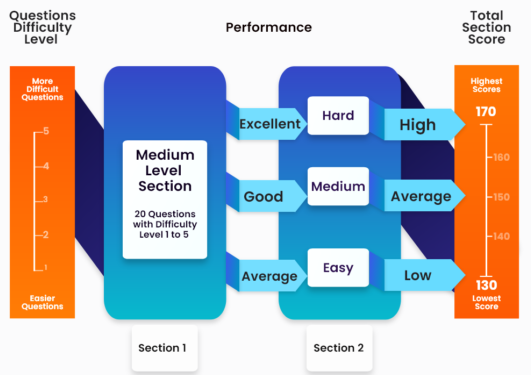
\includegraphics[width=0.9\linewidth]{GRE_Section_Adaptive.png}
	\end{figure}
\end{frame}

%------------------------------------------------
%------------------------------------------------
\subsection{Scoring}

\begin{frame}
	\frametitle{Diagnostic Report 诊断报告}
	\framesubtitle{正常15天出分,出分后3天出诊断报告}
	
	\begin{figure}
		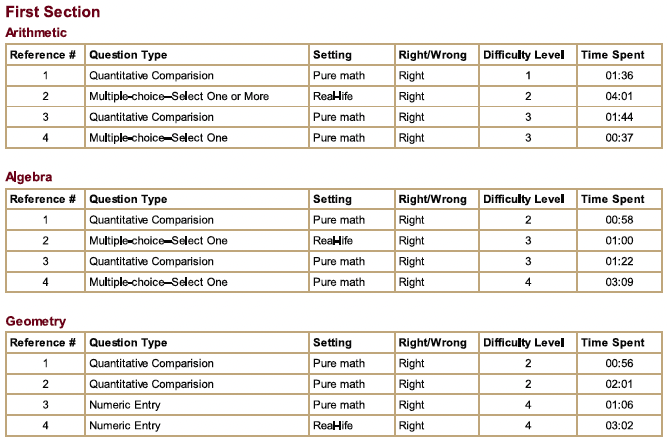
\includegraphics[width=0.9\linewidth]{Diagnostic_Report_Section1_1.png}
	\end{figure}
\end{frame}

%------------------------------------------------

\begin{frame}
	\frametitle{Diagnostic Report 诊断报告}
	\framesubtitle{Data Analysis 用时更多}
	
	\begin{figure}
		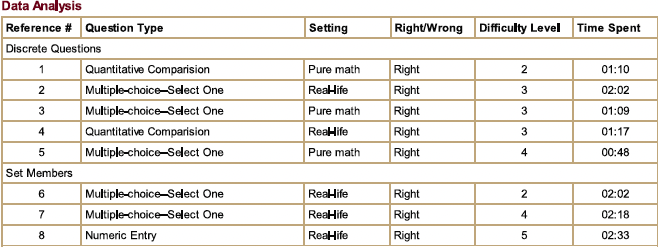
\includegraphics[width=0.9\linewidth]{Diagnostic_Report_Section1_2.png}
	\end{figure}
\end{frame}

%------------------------------------------------

\begin{frame}
	\frametitle{Diagnostic Report 诊断报告}
	\framesubtitle{Section 2 的题目更难}
	
	\begin{figure}
		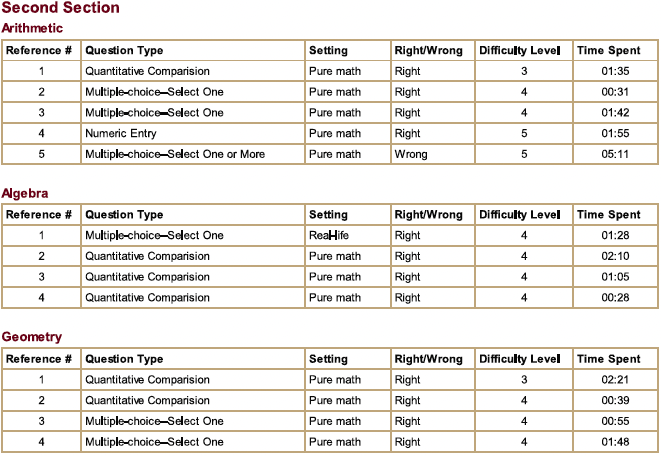
\includegraphics[width=0.9\linewidth]{Diagnostic_Report_Section2_1.png}
	\end{figure}
\end{frame}

%------------------------------------------------

\begin{frame}
	\frametitle{Diagnostic Report 诊断报告}
	\framesubtitle{不定项选择题最容易错}
	
	\begin{figure}
		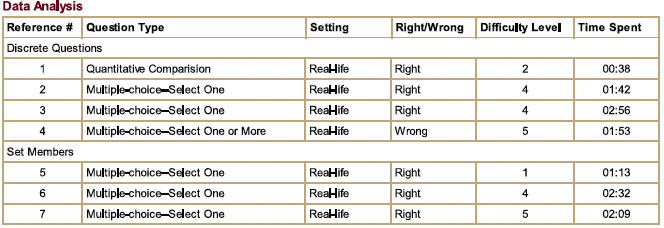
\includegraphics[width=0.9\linewidth]{Diagnostic_Report_Section2_2.png}
	\end{figure}
\end{frame}

%------------------------------------------------

\begin{frame}
	\frametitle{Predict Your Score}
	\framesubtitle{第二个section 错题和分数的关系:错1-2 个170/169}
	
	\begin{figure}
		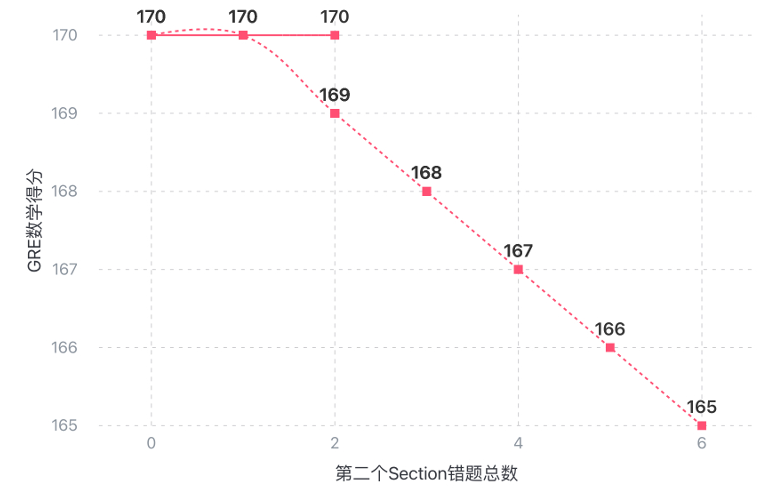
\includegraphics[width=0.9\linewidth]{scoring.png}
		\caption{Regression between the number of incorrect question of the 2nd section and the final score in 38 diagnostic reports}
	\end{figure}
\end{frame}

%------------------------------------------------





%------------------------------------------------
\subsection{Question Types}


\begin{frame}
	\frametitle{Quantitative Comparison 比大小}
	\framesubtitle{选项固定,带入数,估算,化简}
	
	\begin{figure}
		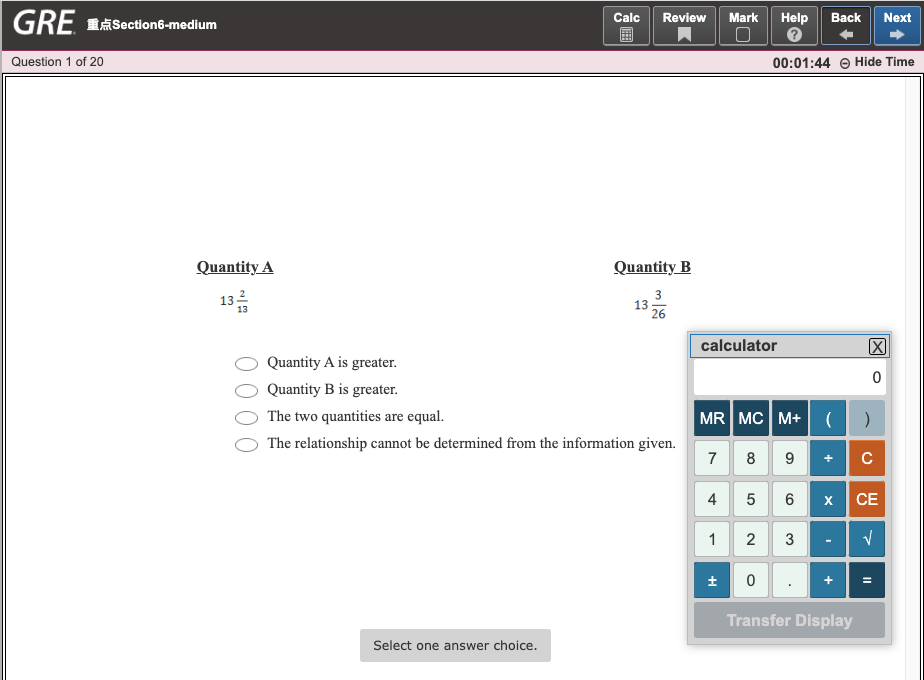
\includegraphics[width=0.9\linewidth]{Quantitative_Comparison.png}
	\end{figure}
\end{frame}

%------------------------------------------------

\begin{frame}
	\frametitle{Multiple-choice—Select One 单选}
	\framesubtitle{如果要近似,选项间隔小,一定要用计算器精确计算,最后一步再化简}
	\begin{figure}
		\includegraphics[width=0.9\linewidth]{Multiple-choice_Questions—Select_One.png}
	\end{figure}
\end{frame}
%------------------------------------------------

\begin{frame}
	\frametitle{Multiple-choice Questions—Select One or More Answer Choices 选一个或者多个,最后一题难度为5}
	\begin{figure}
		\includegraphics[width=0.8\linewidth]{Multiple-choice Questions—Select_One_or_More_Answer_Choices.png}
	\end{figure}
\end{frame}
%------------------------------------------------

\begin{frame}
	\frametitle{Numeric Entry Questions 数字填空题}
	\framesubtitle{注意单位;近似精度;Transfer Display;只能填一个整数或者分数}
	\begin{figure}
		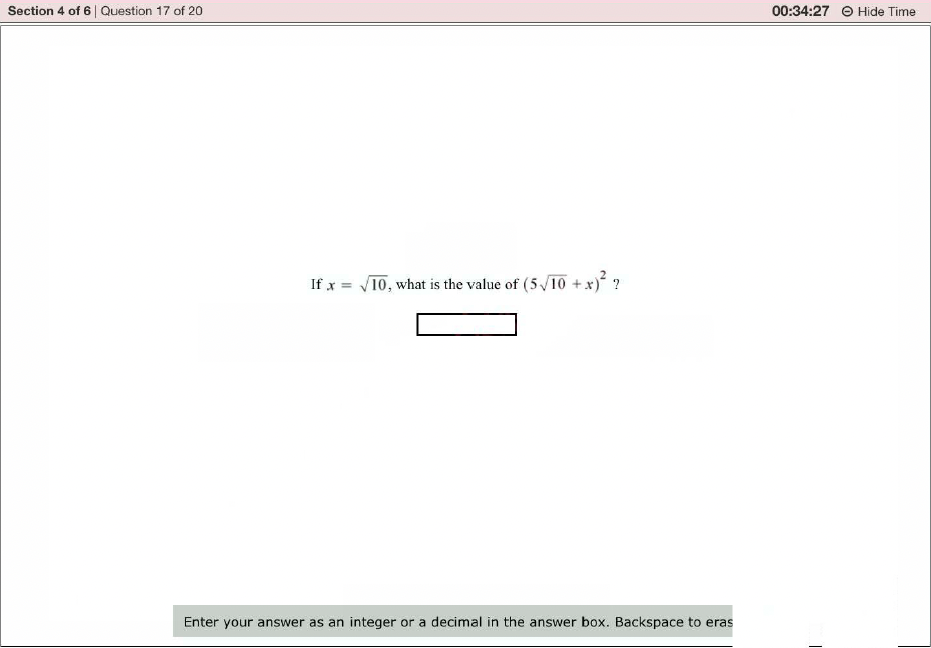
\includegraphics[width=0.9\linewidth]{Numeric_Entry_Questions.png}
	\end{figure}
\end{frame}
%------------------------------------------------

\begin{frame}
	\frametitle{Numeric Entry Questions 数字填空题}
	\framesubtitle{不用化简;分子 分母分开填;}
	\begin{figure}
		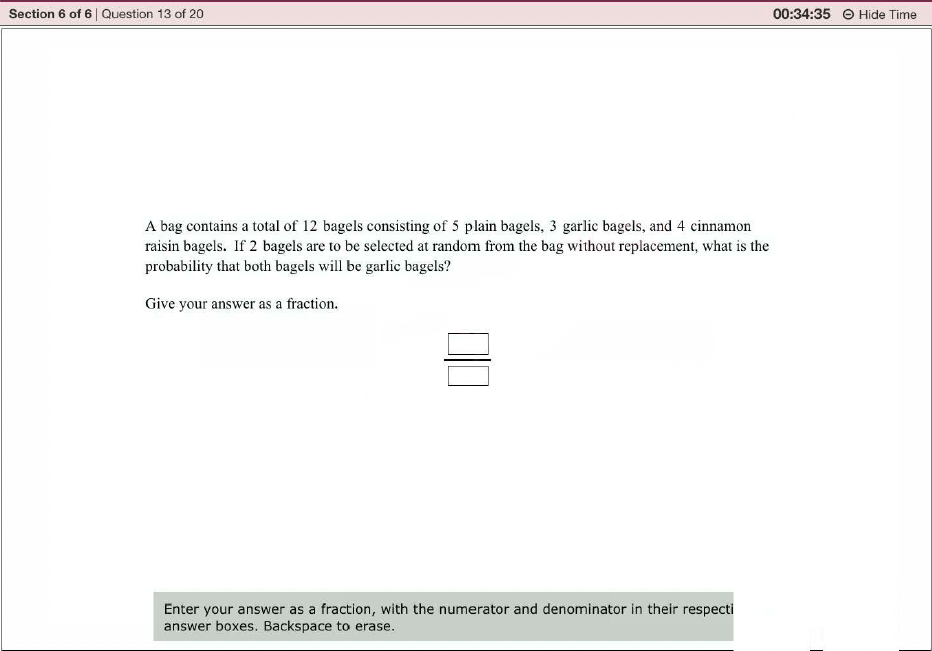
\includegraphics[width=0.9\linewidth]{Numeric_Entry_Questions2.png}
	\end{figure}
\end{frame}
%------------------------------------------------

\begin{frame}
	\frametitle{Data Interpretation Sets 数据解读题套题}
	\framesubtitle{多道题目对应一组数据;可单选,不定项,或者填空}
	\begin{figure}
		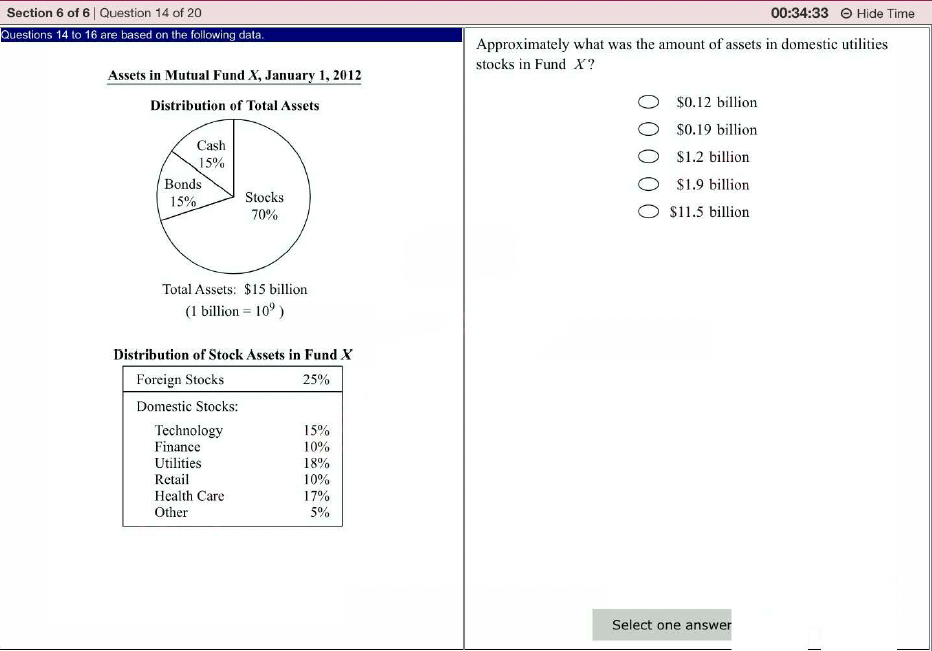
\includegraphics[width=0.9\linewidth]{Data_Interpretation_Sets.png}
	\end{figure}
\end{frame}
%------------------------------------------------

\subsection{How to Use the On-screen Calculator}

\begin{frame}
	\frametitle{When to Use the Calculator}
	\framesubtitle{For tedious calculation only}
	\begin{columns}
		\begin{column}{0.5\textwidth}
			\begin{figure}
			    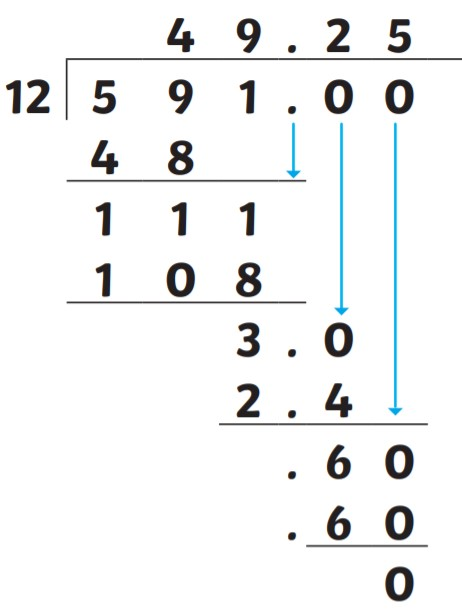
\includegraphics[width=0.7\linewidth]{Long_Division.jpeg}
			    \caption{Long Division}
		    \end{figure}
		\end{column}

		\begin{column}{0.5\textwidth}
		    \begin{itemize}
				\item Long division
				\item Square roots
				\item Addition, subtraction or multiplication of numbers that have several digits
		    \end{itemize}
		\end{column}
	\end{columns}
\end{frame}
%------------------------------------------------

\begin{frame}
	\frametitle{When to \alert{Not} Use the Calculator}
	\begin{columns}[t]
		\begin{column}{0.33\textwidth}
			\textbf{Simple Calculations}
			\begin{enumerate}
				\item $10 - 490$
				\item $ 4 \times 70 $
				\item $\frac{4300}{10}$
				\item $\sqrt{25}$
				\item $30^2$
			\end{enumerate}
		\end{column}

		\begin{column}{0.5\textwidth}
		    \textbf{Fraction}\\
		    Avoid using it to introduce decimals if you are asked to give an answer as a fraction.\\
		   \begin{figure}
			    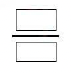
\includegraphics[width=0.3\linewidth]{Numeric_Entry_Questions_Fraction.png}
			    \caption{Numeric Entry Question For a Fraction}
		    \end{figure}
		\end{column}
	\end{columns}
\end{frame}
%------------------------------------------------

\begin{frame}
	\frametitle{Demo: 请打开以下网址}
	\framesubtitle{群内有链接,建议用电脑打开,用小键盘或者鼠标操作}
	\url{https://tonypottera24.github.io/gre_calculator/web/}
	\begin{figure}
			    
\includegraphics[width=0.5\linewidth]{GRE_Calculator.png}
			    \caption{GRE Calculator Website}
		    \end{figure}
	
\end{frame}

%------------------------------------------------

\begin{frame}
	\frametitle{Demo: Order of Operations 运算优先级}
		\textbf{From the Most Prioritized to Least Prioritized}
		\begin{enumerate}
			\item Parentheses
			\item Exponentiation (including square roots)
			\item Multiplications and divisions (from left to right)
			\item Additions and subtractions (from left to right)
		\end{enumerate}

		\bigskip
	    \textbf{Have a try!}\\
			\begin{itemize}
				\item $1 + 2 \times 4 = 9$   
				\item $(1 + 2) \times 4 = 12$
				\item $7 + (3 \times 15 - 5) \div 8 - 13 = ?$
			\end{itemize}
			\bigskip
		\fbox{CE}: Clear Entry 清零屏幕上所有输入  \\
		\fbox{C}: Clear 清零之前所有输入
\end{frame}

%------------------------------------------------

\begin{frame}
	\frametitle{Demo: Memory Buttons}
	\begin{columns}[t]
			\begin{column}{0.2\textwidth}
				\textbf{Buttons}
				\begin{enumerate}
				\item \fbox{MR}: Memory Recall
				\item \fbox{MC}: Memory Clear
				\item \fbox{M+}: Memory Plus
			\end{enumerate}
			\end{column}

			\begin{column}{0.8\textwidth}
			   \begin{figure}
				    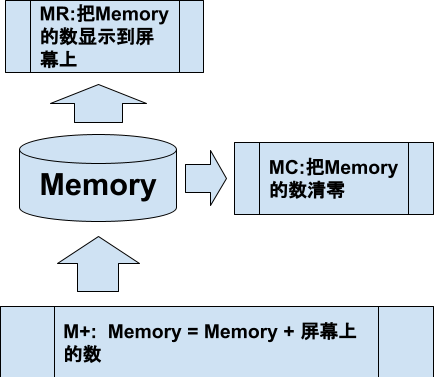
\includegraphics[width=0.7\textwidth]{Memory_Buttons_How.png}
				    \caption{How \fbox{MR}, \fbox{MC}, \fbox{M+} works}
			    \end{figure}
			\end{column}
		\end{columns}
\end{frame}

%------------------------------------------------

\begin{frame}
	\frametitle{Demo: Memory Buttons}
	\begin{columns}[t]
	        \begin{column}{0.5\textwidth}
	        \textbf{Have a try!}
		        \begin{enumerate}
					\item If a car run 33 miles with 20 gallons gas, how many gallons will the car use for 1 mile? With 45 gallons of gas, how many miles can the car run? 
					\item Convert this fraction to decimal. $\frac{43 \times 6 + 21 \times 80 + 16 \times 100}{43 + 21 + 16}$
					\item Calculate the Standard Deviation of ages for Alice(56 years-old) and Bob(73 years-old).
				   \end{enumerate}
			\end{column}

			\begin{column}{0.5\textwidth}
			   \begin{figure}
				    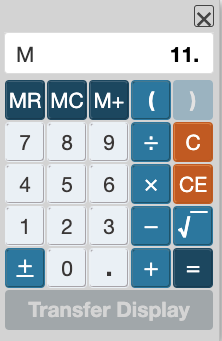
\includegraphics[width=0.5\textwidth]{Memory_Buttons.png}
				    \caption{The "M" symbol will appear on the left of the display.}
			    \end{figure}
			\end{column}
	\end{columns}
\end{frame}

%------------------------------------------------

\begin{frame}
	\frametitle{Demo: the Mysterious "$\pm$"}
	\framesubtitle{不是加减,而是负号}
	\begin{columns}[t]
				\begin{column}{0.5\textwidth}
			   "$\pm$" \alert{dose not} suggest that the calculator will perform the plus and minus operation at the same time. \\
			    "$\pm$" suggest  a negative sign is added to the number on the display. 
			  \end{column}

	        \begin{column}{0.5\textwidth}
	          \textbf{Have a try!}
		        \begin{enumerate}
							\item Compute $-\frac{8.4 + 9.3}{70}$: \\ \fbox{(} 8.4 \fbox{+} 9.3 \fbox{)} \fbox{$\div$} 70 \fbox{=} \fbox{$\pm$}
							\item Compute $(-15)^3$: \\ 15 \fbox{$\times$} 15 \fbox{$\times$} 15 \fbox{=} \fbox{$\pm$}
				   \end{enumerate}
					\end{column}
	\end{columns}
\end{frame}

%------------------------------------------------


\begin{frame}
	\frametitle{Demo: The Square root}
	\framesubtitle{先得出数字,然后按$\sqrt{}$}
	\begin{columns}[t]
				\begin{column}{0.5\textwidth}
				Find the length, to the nearest 0.01, of the hypotenuse of a right triangle with legs of length 21 and 54; 
			  \end{column}

	        \begin{column}{0.5\textwidth}
						 Compute $\sqrt{21^2 + 54^2}$: \\ 21 \fbox{$\times$} 21 \fbox{+} 54\fbox{$\times$} 54 \fbox{$=$} \fbox{$\sqrt{}$} 
					\end{column}
	\end{columns}
\end{frame}

%------------------------------------------------
\begin{frame}
	\frametitle{Demo: Deal with Error}
	\framesubtitle{按\fbox{C};减小运算位数}
	\begin{columns}[t]
				\begin{column}{0.3\textwidth}
			   \begin{figure}
				    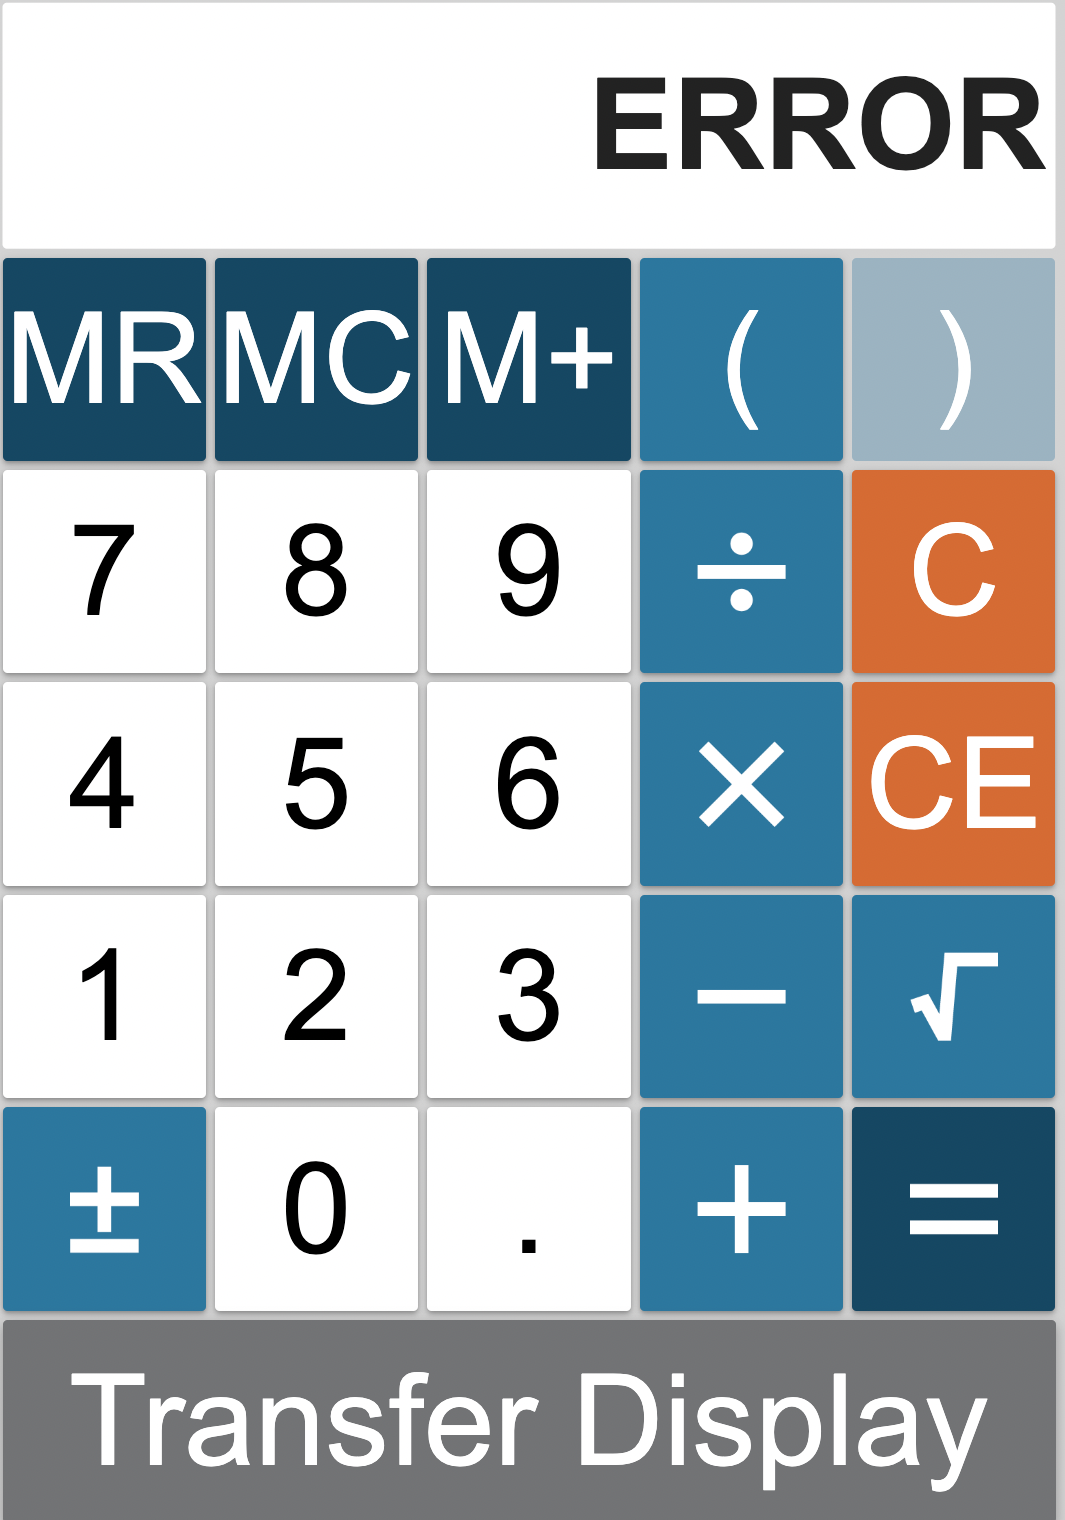
\includegraphics[width=0.3\textwidth]{GRE_Calculator_Error.png}
				    \caption{The error on the display}
			    \end{figure}
			\end{column}
			
	        \begin{column}{0.7\textwidth}
	        \textbf{Why do you  got an error?}
		        \begin{itemize}
							\item Undefined Behaviors For Real Numbers
							\begin{itemize}
								\item Divided by zero:\\ 6 \fbox{$\div$}0 \fbox{=} \textbf{Error}
								\item The Square root of a negative:\\ 7 \fbox{$\pm$} \fbox{$\sqrt{}$}  \textbf{Error}
							\end{itemize}
							\item The 8-Digits Limit
							\begin{itemize}
								\item 99,999,999 is the maximum allowable number:\\ 10000000 \fbox{$\times$} 10 \fbox{=} \textbf{Error}
								\item 0.0,000,001 is the minimum positive number: 0.0000001 \fbox{$\div$} 10 \fbox{=} 0.
							\end{itemize}
				   \end{itemize}
			\end{column}
	\end{columns}
	\bigskip
	Incomplete brackets will not cause an error. 1 \fbox{+} \fbox{$($} 10 \fbox{=} 11
\end{frame}

%------------------------------------------------

\begin{frame}
	\frametitle{Use the Calculator}
	\begin{figure}
		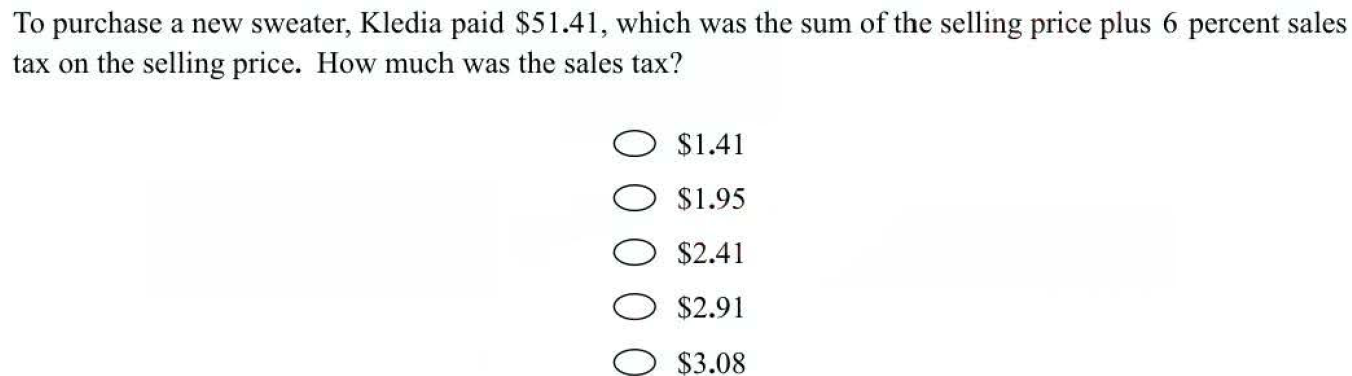
\includegraphics[width=\linewidth]{Calculator_Example_2.png}
	\end{figure}
	\pause
	51.41 \fbox{$\div$} \fbox{(} 1 \fbox{+} 0.06 \fbox{)} \fbox{$\times$} 0.06 \fbox{=} 2.91  D
\end{frame}

%------------------------------------------------

\begin{frame}
	\frametitle{Don't Use the Calculator!}
	\begin{figure}
		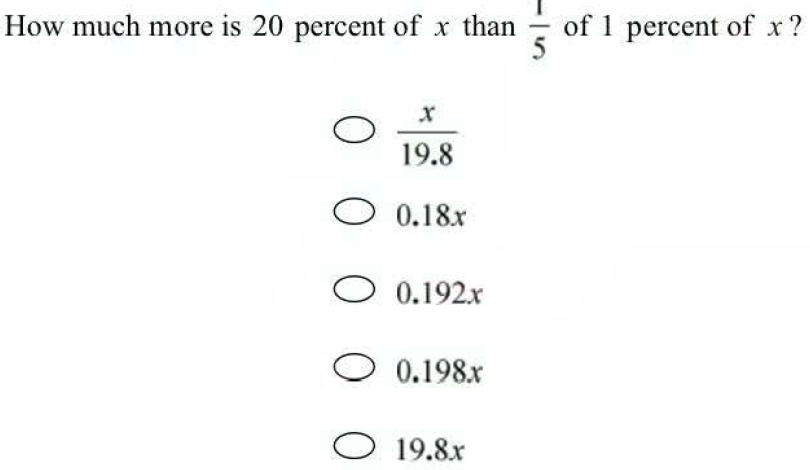
\includegraphics[width=\linewidth]{Calculator_Example_1.png}
	\end{figure}
	\pause
	$0.2 - 0.2 \times 0.01 = 0.198$ D
\end{frame}

%------------------------------------------------
\begin{frame}
	\frametitle{A Sneak Peak}
	\begin{enumerate}
		\item {\LARGE Arithmetic 算术}
		\item {\LARGE Algebra 代数} 
		\item {\LARGE Geometry 几何}
		\item {\LARGE Data Analysis 数据分析}

	\end{enumerate}
\end{frame}

%------------------------------------------------

%----------------------------------------------------------------------------------------
%	CLOSING SLIDE
%----------------------------------------------------------------------------------------

\begin{frame}[plain] % The optional argument 'plain' hides the headline and footline
	\begin{center}
		{\Huge 1 Min Break}
		\bigskip\bigskip % Vertical whitespace
		
		{\LARGE Questions? Comments?}
	\end{center}
\end{frame}

%----------------------------------------------------------------------------------------

\end{document} 